\begin{blocksection}

\question
Implement \textbf{movz} (but not movnz) in the datapath. Choose the correct implementation for (a), (b), and (c). Note that you do not need to use all the signals provided to each box, and the control signal MOVZ is 1 if and only if the instruction is \textbf{movz}. In the following diagrams, RF[rs] refers to R[rs1] and RF[rt] refers to R[rs2]. ALUZero = 1 if the A input of the ALU is zero.


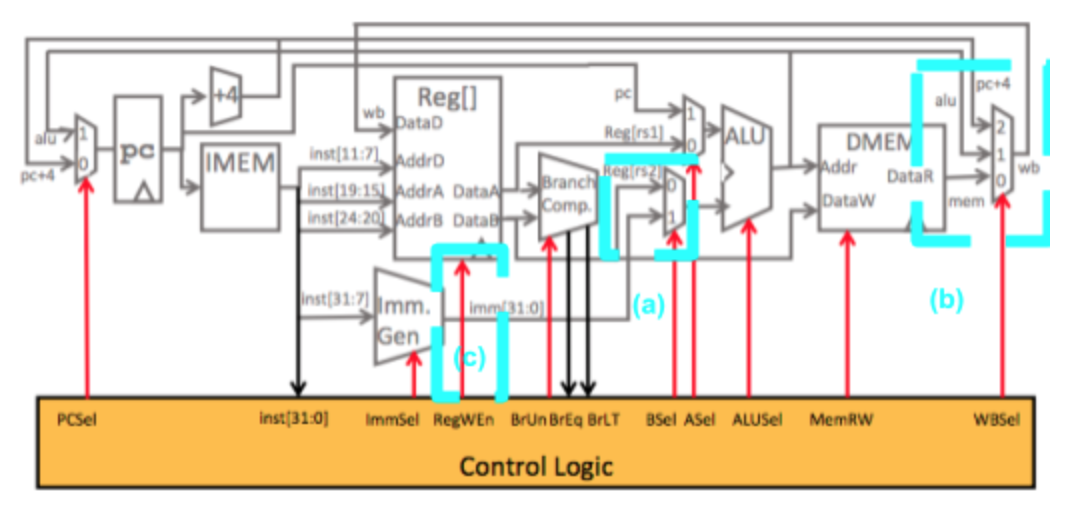
\includegraphics[width=\textwidth]{images/singlecycle/movz_1.png}
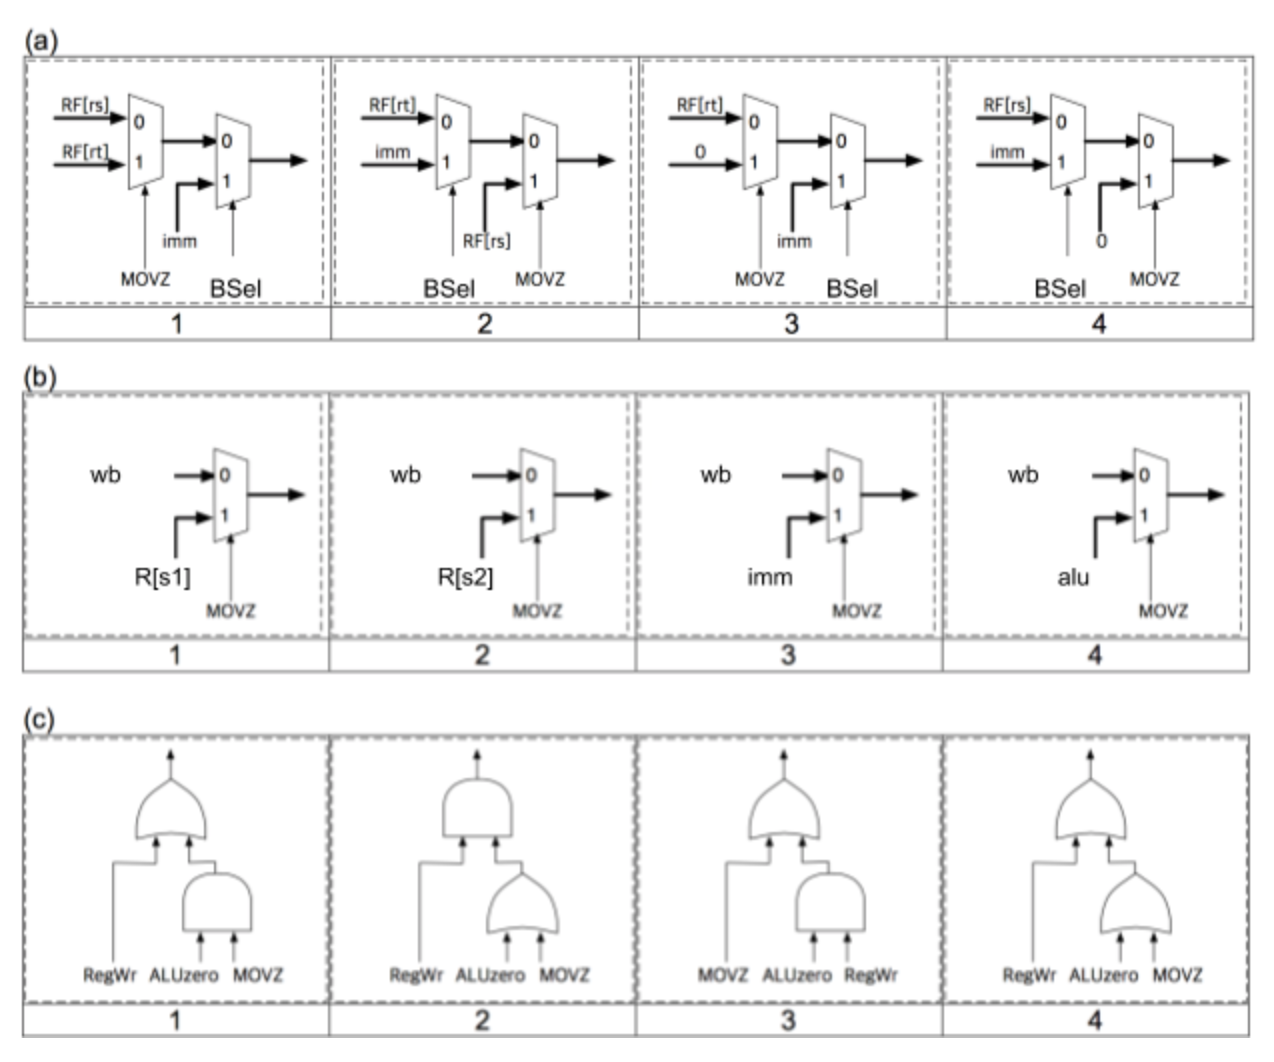
\includegraphics[width=\textwidth]{images/singlecycle/movz_2.png}


\begin{solution}[0.5in]
 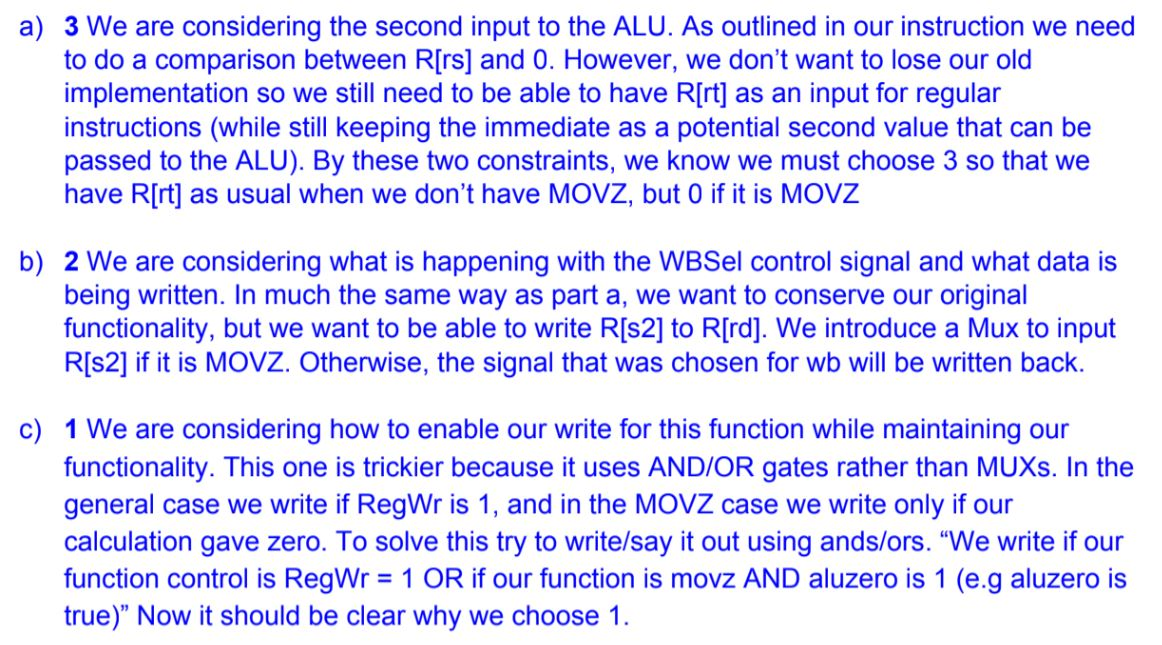
\includegraphics[width=\textwidth]{images/singlecycle/movz_2_sol.png}
\end{solution}

\end{blocksection}